\documentclass[presentation]{subfiles}

\onlyinsubfile{
\bibliography{references}
  % \beamertemplategridbackground[1mm]
}


\begin{document}

\section{Complexity}

\begin{frame}{Complexity}
  What kinds of problems do we mean when we talk about complexity?
  \begin{itemize}
    \item<1-> Can crowds help you write something?
    
    \scriptsize{
      \textcite{bernsteinSoylent,Kim:2014:CSI:2556288.2556986,Nebeling:2016:WCW:2858036.2858169}
    }
    \item<2-> Can crowds critique novel designs?
    
    \scriptsize{
      \textcite{yuanAlmost,fuge2014analysis}
    }
    \item<3-> Can crowds create things from whole cloth?
    
    \scriptsize{
      \textcite{KimStoria,Kim2017,Hahn:2016:KAB:2858036.2858364,Lasecki:2014:LSR:2661334.2661352}
    }
  \end{itemize}
\end{frame}


\begin{frame}{What does the crowdsourcing literature say?}
\begin{columns}
  \begin{column}{0.6\textwidth}
    \begin{itemize}
      \item Build complexity into the process
      \begin{mystepwiseitemize}
        \item Apply CS methods to people

        \scriptsize{
          \textcite{crowdForgeKittur}
        }
        \item Humans as computational units

        \scriptsize{
          \textcite{Lasecki:2014:LSR:2661334.2661352}
        }
        \item Crowdsourcing workflows as function state machines

        \scriptsize{\textcite{latoza2014microtask}
        }
      \end{mystepwiseitemize}
    \end{itemize}
  \end{column}
  
  \begin{column}{0.4\textwidth}
    \begin{figure}
    \only<1>{
    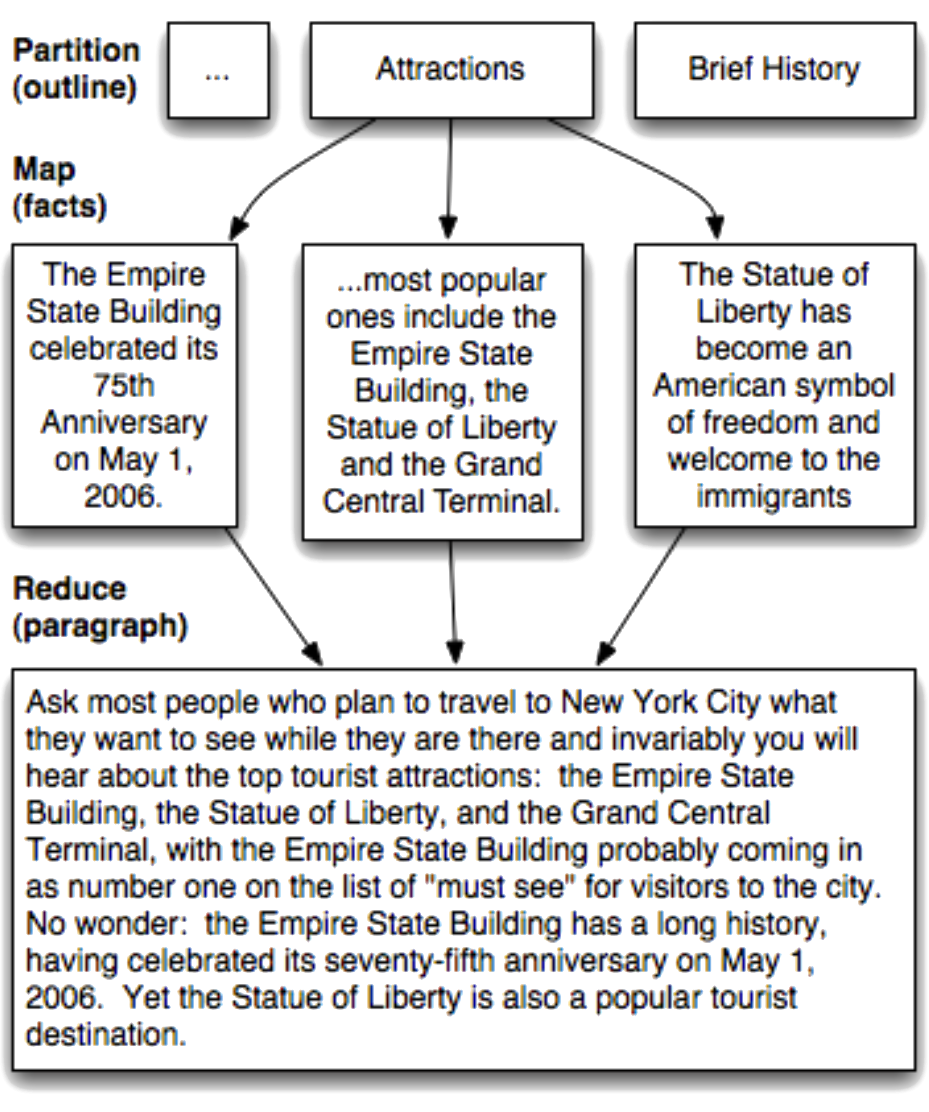
\includegraphics[width=\textwidth]{figures/complexity/cw_literature/mapReduce.png}
    }
    
    \only<2>{
      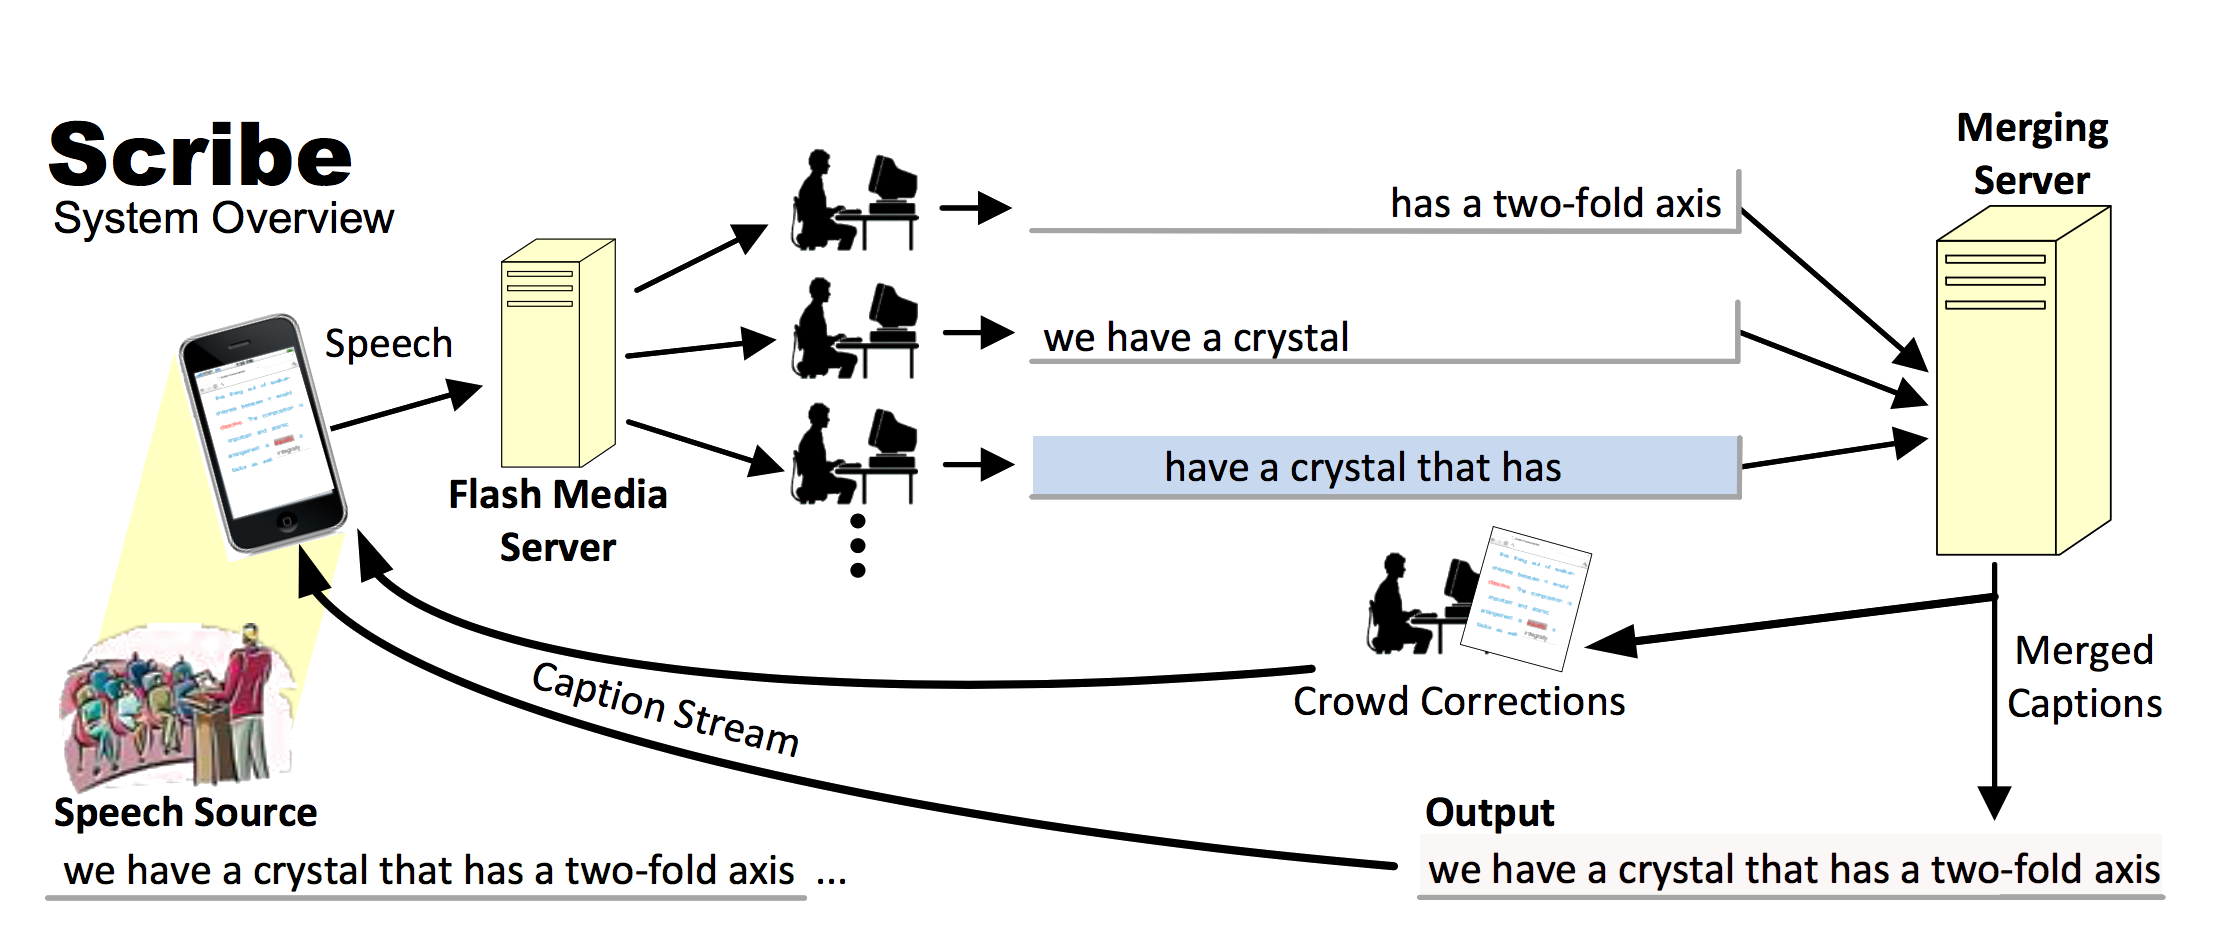
\includegraphics[width=\textwidth]{figures/complexity/cw_literature/scribe.png}
    }
    \only<3>{
      \begin{adjustbox}{max totalsize={\textwidth}{\textheight},center}
      \begin{tikzpicture}[->,>=stealth',auto, node distance=4cm,
                          thick,transform shape]
        \node[state,label=above:{Described}]                       (A)                    {};
        \node[state,label=left:{Described written}]                (B) [below of=A]       {};
        \node[state,label=left:{Run Tests}]                        (D) [below of=B]       {};
        \node[state,label=below:{Described written buggy}]         (C) [below right of=D] {};
        \node[state,label=below:{Described written buggy}]         (E) [below left of=D]  {};

        \path[every node/.style={sloped,anchor=south}]
              (A) edge              node {Write description} (B)
              (B) edge [loop right] node {Edit code} (B)
                  edge              node {Edit code} (D)
              (D) edge              node {} (C)
                  edge              node {} (E)
              (C) edge [bend right] node {Debug} (B)
                  edge [bend right] node {Debug} (D)
              (E) edge [bend right] node {Edit Code} (D)
                  edge [bend left]  node {Edit Code} (B);
        \end{tikzpicture}
        \end{adjustbox}
    }
    \end{figure}
  \end{column}
  
\end{columns}
\end{frame}

\begin{frame}{What does the piecework literature say?}
    % \begin{itemize}
      % \item
      George Airy (astronomer) used a very similar approach~\cite{grier2013computers}
      % \begin{itemize}
      %   \item Break work up so that individual tasks are simple

      %   Make the process \textit{itself} compile the final product.
      % \end{itemize}
    % \end{itemize}
    % \vspace{0mm}
    \begin{columns}
    \begin{column}{0.6\textwidth}
      \begin{figure}
        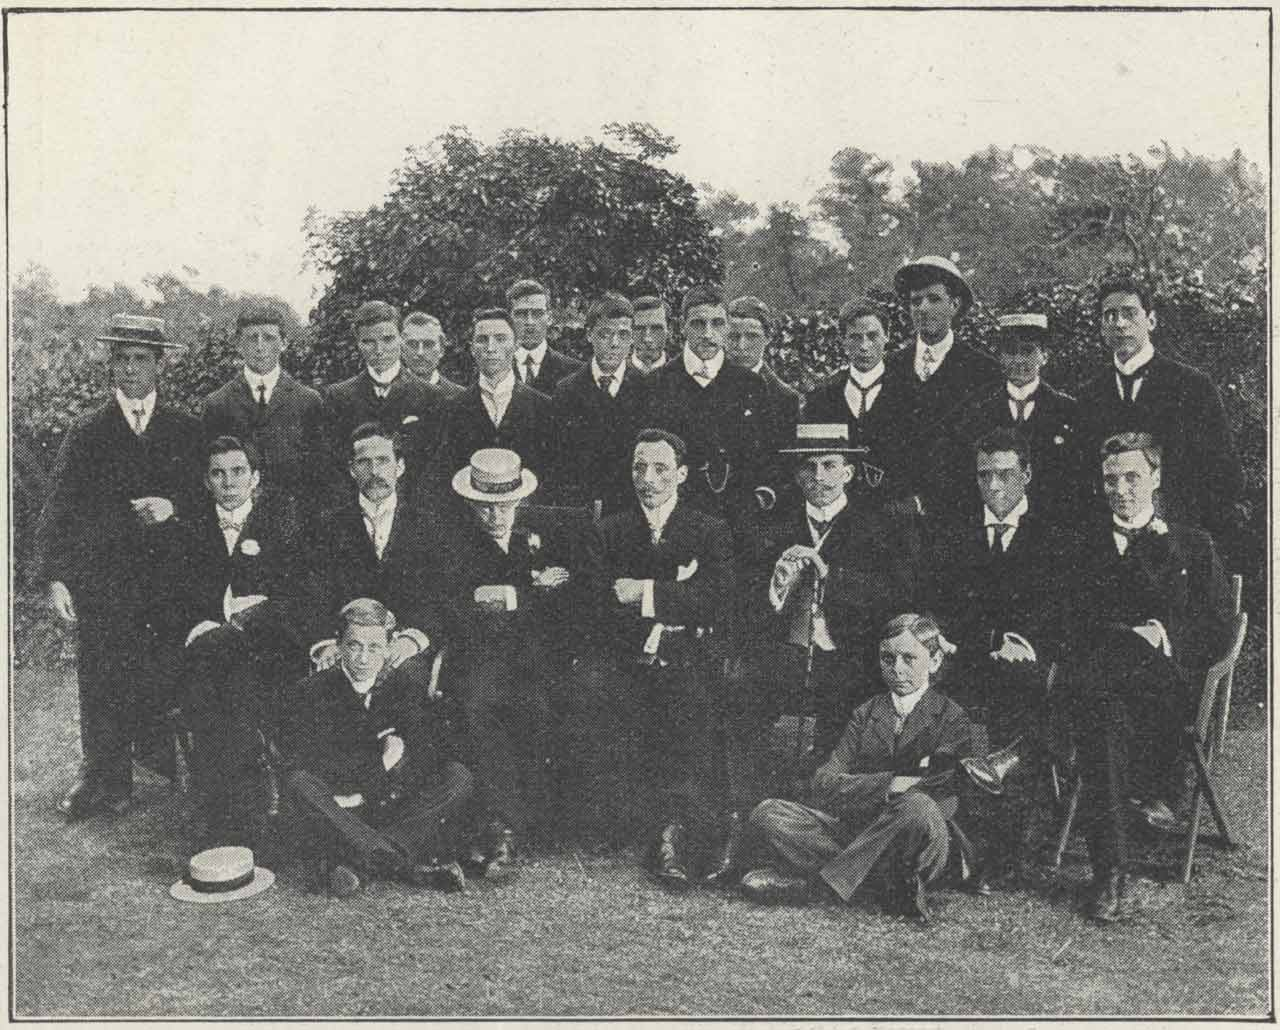
\includegraphics[width=\textwidth]{figures/photo/Greenwich-Observatory-computing-staff-1902.jpg}
      \end{figure}
    \end{column}
    
    \begin{column}{0.4\textwidth}
      \begin{itemize}
        \item Employed computers
        \item 13--20 years old
        \item Overworked
        \item Underpaid
        \item Could be fired at will
      \end{itemize}
    \end{column}
    \end{columns}

\end{frame}


\begin{frame}{George Airy --- whiz kid}
    Airy built complexity into the process, assigning \textit{human computers} 
    to compute, verify, and correct the right ascension and declination of stars.

    \begin{figure}
    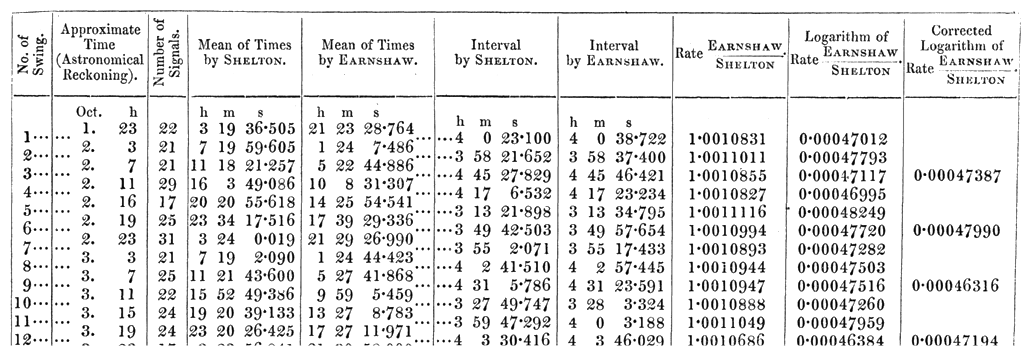
\includegraphics[width=\textwidth]{figures/complexity/pw_literature/airy.png}
    \end{figure}
\end{frame}

\begin{frame}{Humble origins}
  First implementations of piecework:
  \visible<2->{farms}\visible<3->{, textiles}\visible<4->{, and other low--skill labor.}
  \begin{columns}
  
  \visible<2->{
  \begin{column}{0.3\textwidth}
  \begin{figure}
  
\includegraphics[width=\textwidth]{figures/idk.png}
  \end{figure}
  \end{column}
  }
  
  \visible<3->{
  \begin{column}{0.3\textwidth}
  \begin{figure}
  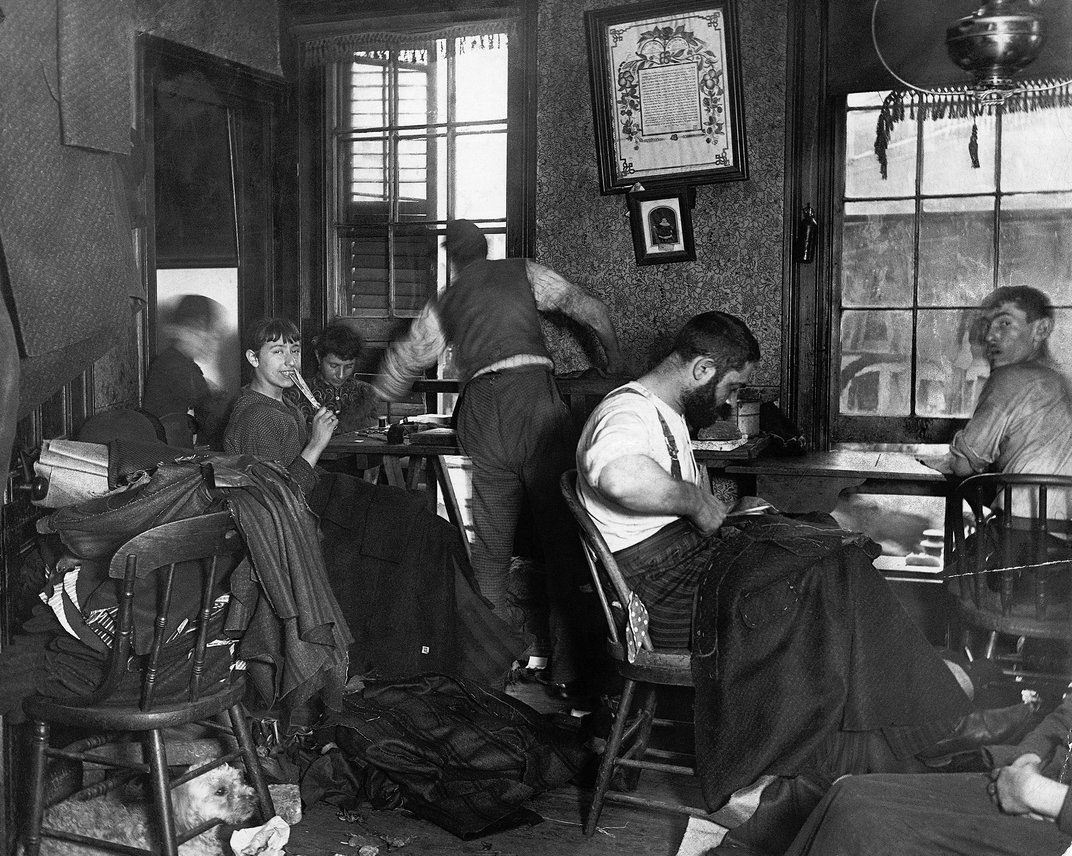
\includegraphics[width=\textwidth]{figures/pieceworkers.jpg}
  \end{figure}
  \end{column}
  }
  
  \visible<4->{
  \begin{column}{0.3\textwidth}
  \begin{figure}
  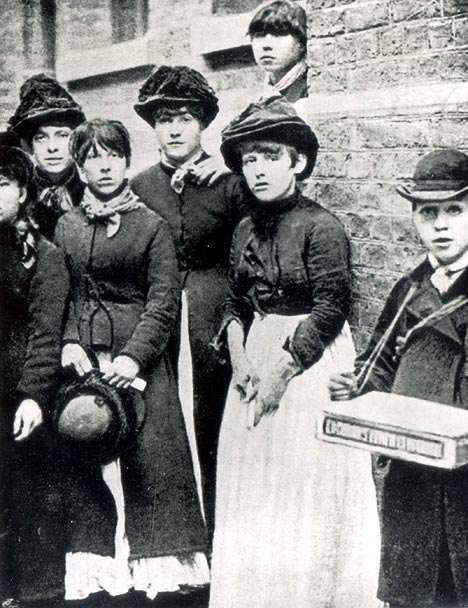
\includegraphics[width=\textwidth]{figures/photo/Matchgirl_strikers.PNG}
  \end{figure}
  \end{column}
  }
  \end{columns}
\end{frame}

\begin{frame}{Ford}
    Fordism


\end{frame}

\begin{frame}{Comparisons}
% \framesubtitle{something else}
%   \begin{columns}
%   \begin{column}{0.5\textwidth}
%   % \section*{Piecework}
%      some text here some text here some text here some text here some text here

%   \end{column}

%   \begin{column}{0.5\textwidth}
%   % \section*{CrowdWork}
%      some text here some text here some text here some text here some text here

%   \end{column}
%   \end{columns}
\end{frame}

\onlyinsubfile{
  \printbibliography{}
}
\end{document}